\section{Hyper-optimization}
\label{sec:hyper-opt}

We want to address the problem of finding the minimum of an {\em unknown}\ function $f$,
\begin{equation}
    \label{eq:FDef}
    f: \Omega \to \mathbb{R}\, ,
\end{equation} 
where $\Omega$ is a compact subset of $\Rd$. Although $f$ is unknown, we assume
that we can perform {\em noisy}\ estimates of $y=f(x)$ for given values of $x$,
such that
\begin{equation}
    \label{eq:UnbiasedEval}
    \Ebb\left[y|f(x)\right] = f(x)\, ,
\end{equation}
where the average here is over the fluctuations of $y$. Our knowledge of the function $f$ is encoded in the probability distribution function of $f(x)$ for each value of $x$. At the beginning of the process we need to choose a prior distribution for these values. The prior distribution is then updated according to the value of noisy measurements of $f$ at given values of $x$.  

Bayesian Optimization is an algorithm that performs a sequential search by
selecting at every step a position $x$ in $\Omega$ according to some acquisition
function, and computing the corresponding value of $y$. After $\nopt$ iterations
the algorithm yields its current best estimate of the position of the minimum.
The procedure is summarised in Fig.~\ref{fig:BOpt}, taken from
Ref.~\cite{Shahriari}.

\begin{figure}[ht!]
    \label{fig:BOpt}
    \centering
    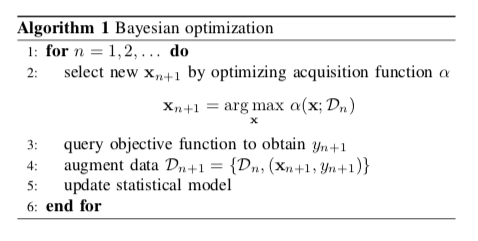
\includegraphics[scale=0.5]{BayesianOptAlg.png}
    \caption{\small Summary of the Bayesian Optimization procedure.}
\end{figure}

\paragraph[]{Summary} The important ingredients in BO are the following. 
%
\begin{enumerate}
    \item[$\bullet$] Choice of the space of parameters, which we denoted $\Omega$ above.  
    \item[$\bullet$] Choice of the loss function $f$, and methodology to evaluate it. 
    \item[$\bullet$] Update of the prior distribution for $f(x)$.
    \item[$\bullet$] Choice of the acquisition function $\alpha$.
    \item[$\bullet$] Choice of the value of $x$ for a new measurement, given the acquisition function.   
\end{enumerate}
%
We need to specify each of these steps in our procedure. 


\subsection{Parametric Models}
\label{sec:BaysParMod}

There are interesting results on parametric models, which are useful to
understand the idea behind BO. In parametric models the function $f$ is
specified by a set of parameters $w$. The current knowledge of $f$ is then
encoded in the probability distribution of these parameters. 

\paragraph[]{Explicit Examples}

\subsection{Non-parametric Models}
\label{sec:BaysNonParMod}

A Gaussian Process $\mathrm{GP}(\mu, k)$ is fully characterised by its mean
function $\mu: \Omega\to \Rbb$, and its kernel function $k: \Omega \times \Omega
\to \Rbb$. We are going to use a Gaussian Process to define the prior for the
unknown function $f$. For a collection of points $\{x_i, i=1,\ldots,n\}$, we
have a set of values $\{f_i=f(x_i), i=1,\ldots,n\}$ and their noisy estimates
$\{y_i, i=1\ldots, n\}$. Remember that $x_i\in\Omega$ is a $d$-dimensional real
vector for every value of $i$. Their respective distributions will be: 
\begin{align}
    \label{eq:GPone}
    \mathbf{f}|\mathbf{x} &\sim 
        \mathcal{N}\left(\mathbf{m},\mathbf{K}\right)\, ,\\
    \mathbf{y}|\mathbf{f},\sigma &\sim 
        \mathcal{N}\left(\mathbf{f},\sigma^2\right)\, ,
\end{align}
where $m_i=\mu(x_i)$ and $K_{ij}=k(x_i,x_j)$. In Eq.~\eqref{eq:GPone} we denote
by boldface fonts vectors and matrices in the $n$-dimensional space of
measurements that have been performed. 

After $n$ observations $\mathcal{D}_n=\left\{\left(x_i,y_i\right)\right\}$, the random variable $f(x)$ is Gaussianly distributed, 
\begin{equation}
    \label{eq:PostGaussF}
    f(x)\sim \mathcal{N}\left(\mu_n(x),\sigma_n(x)\right)\, ,
\end{equation}
with
\begin{align}
    \label{eq:PostParams}
    \mu(x) &= \mu(x) + \mathbf{k}(x)^T \left(\mathbf{K} + \sigma^2 \mathbf{I}\right)^{-1} \left(\mathbf{y}-\mathbf{m}\right)\, , \\
    \sigma(x)^2 &= k(x,x) - \mathbf{k}(x)^T \left(\mathbf{K} + \sigma^2 \mathbf{I}\right)^{-1} \mathbf{k}(\mathbf{x})\, .
\end{align}
This posterior distribution encodes our knowledge of the function $f$ at a
generic point $x\in\Omega$. It is then used to select the next point in the
search. 

\subsection{Acquisition Function}
\label{sec:AcqFun}

In BO the choice of the next point $x$ where the function $f$ is going to be
evaluated plays a crucial role. Choosing a random point would be extremely
inefficient, especially if the dimensionality of the space is increased. 

An informed choice of the point $x$ can be made from the knowledge of the
posterior distribution of $f$, and a utility function $U(x,v)$, where $v=f(x)$.
The utility function describes in some sense how much information is provided by
a measurement at $x$. Since $f$ is unknow, we can marginalise with respect to
$v$ using the probability distribution discussed above and define the {\em
expected utility} of a query point:
\begin{equation}
    \label{eq:ExpUtilDef}
    \alpha(x,\mathcal{D}_n) = \Ebb_{v|\mathcal{D}_n}\left[U\left(x,v\right)\right]\, .
\end{equation} 

\paragraph[]{Improvement-based policies}

The acquisition function favours points that are likely to exceed some target value $\tau$; this strategy is called {\em probability of improvement}\ (PI) and for the case of a Gaussian distribution for $f$ we obtain
\begin{equation}
    \label{eq:AlphaPI}
    \alpha_\PI\left(x;\mathcal{D}_n\right) = 
    \Pbb\left[v>\tau\right] = 
    \Phi\left(
        \frac{\mu_n(x)-t}{\sigma_n(x)}    
    \right)\, ,
\end{equation}
where $\Phi$ is the normal cumulative distribution function, \ie\ $\Phi(\zeta)$
is the integral of a Gaussian distribution with unit variance from $-\infty$ to
$\zeta$. This choice corresponds to the utility function
$U(x,v)=\Ibb\left[v>\tau\right]$ being marginalised over $v$.

A similar acquisiton function can be defined trying to quantify the amount of
improvement. In this case the utility function is
\begin{equation}
    \label{eq:EIUtil}
    U(x,v) = (v-\tau) \Ibb\left[v>\tau\right]\, ,
\end{equation}
and the acquisition function is defined as above by taking the expectation value with respect to $v$:
\begin{equation}
    \label{eq:EIAcq}
    \alpha_\EI \left(x;\mathcal{D}_n\right) = 
    \Ebb_{v|\mathcal{D}_n}\left[U(v,x)\right]\, .
\end{equation}
